\section{Matrix Product States (MPS)}


Within a given Hilbert Space, a random state follows a volume law.
In other words, the entanglement entropy of this state grows linearly with the "volume".
For a one-dimensional system the "volume" corresponds to the length of the system. \\

On the other hand, the ground states of a gapped Hamiltonian obey an area law, i.e. the entropy is proportional to the area of the cut that partitions the Hilbert Space.
For a 1D case this implies that the entropy is constant with respect to the increase of the system size $N$. \\

For the random states mentioned previously, the entanglement entropy is close to its maximum value, for which the Schmidt coefficients are close to being constant.
In contrast, the states following an area law (like a ground state) are slightly entangled, which results in most of the weight being distributed in only a few Schmidt coefficients.
This subtle but important observation allows for the introduction of a compressed representation of these "product states" known as: 
matrix-product states (MPS).\\

We consider a one dimensional chain made up of $N$ sites, with each individual site $n$ having a local basis labeled as $\ket{j_n}$ for $j_n = 0, \dots, d$, where $d$ is the dimension of the n$^{th}$ site's Hilbert Space.
The figure below shows a diagrammatic representation of a tensor with $N$ physical legs.

\begin{figure}[h!]
    \centering
    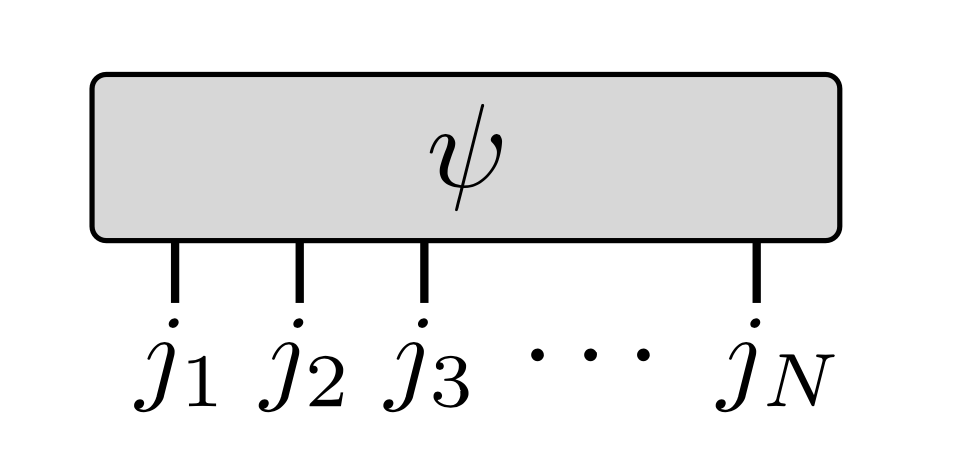
\includegraphics[scale=0.5]{Figures/MPS_1.png}
    \caption{Diagram representation of a $N$ dimensional tensor. Source: \cite{anleitung}}
    \label{fig:mps-1}
\end{figure}

The problem is that even for relatively simple configurations, such as a half spin system, an exact simulation is possible only up to approximately 40 sites \cite{anleitung} due to the exponentially increasing number of entries to store.
This is exactly why MPS representation comes in handy.
A general pure state can be written in MPS as~\cite{anleitung}:

\begin{equation}
    \ket{\Psi} = \sum_{j_1,...,j_N} M^{[1]j_1} M^{[2]j_2} ... M^{[N]j_N} \ket{j_1,j_2,...,j_N}
    \label{eq:MPS_1}
\end{equation}

Where each $ M^{[n]j_n}$ is a $\chi_n \times \chi_{n+1}$ dimensional matrix and $[n]$ tells us that, for a general state, the matrices on each site could be different.
In order to obtain a number as the result of the matrix multiplication, the convention is that $\chi_1 = \chi_{N+1} = 1$, meaning that the first and last matrices are actually vectors.\\

From the superscript $j_n$ we see that there are $d$ matrices corresponding to each site, and these can be grouped to form a 3-degree tensor as shown here:

\begin{figure}[h!]
    \centering
    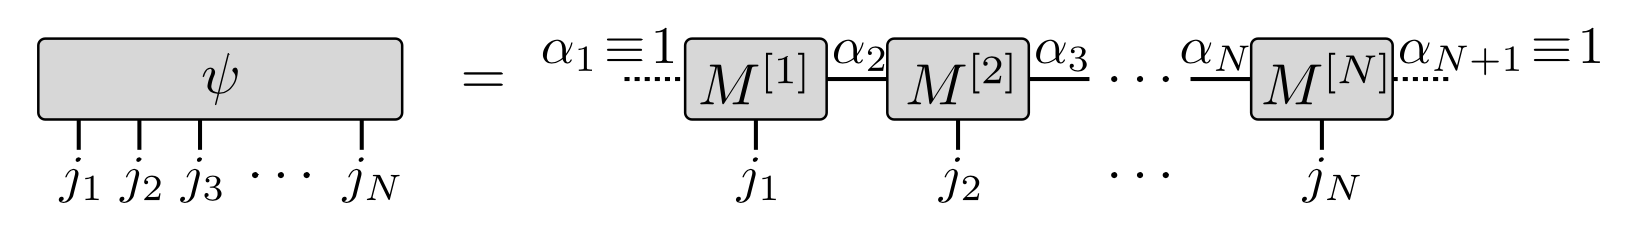
\includegraphics[scale=0.5]{Figures/MPS_2.png}
    \caption{MPS representation of quantum state. Source \cite{anleitung}}
    \label{fig:mps-2}
\end{figure}

Where $\alpha_i$ are the virtual legs or bonds, which are by nature different than the physical indices $j_n$\\

A so called "canonical form" can be defined based on the freedom of choice of the matrices representing our quantum state. This results in the equation \cite{anleitung}:

\begin{equation}
    \ket{\Psi} = \sum_{j_1,...,j_N} \Lambda^{[1]} \Gamma^{[1]j_1}\Lambda^{[2]} \Gamma^{[2]j_2}\Lambda^{[3]}...\Lambda^{[N]} \Gamma^{[N]j_N} \Lambda^{[N+1]} \ket{j_1,j_2,...,j_N}
    \label{eq:mps-canonical}
\end{equation}

Where the matrices $\Lambda^{[n+1]}$ are square diagonal matrices that contain the Schmidt values $\Lambda^{[n+1]}_{\alpha_{n+1}}$ in the diagonal and the $\Gamma^{[n]j_n}$ are such that $\Gamma^{[n]j_n}\Lambda^{[n+1]}$ for each site returns the original state.
This grouping, however, can also be done in two different standard ways:
\begin{equation}
    A^{[n]j_n} = \Lambda^{[n]} \Gamma^{[n]j_n}
    \label{eq:mps-left-canonical}
\end{equation}
\begin{equation}
    B^{[n]j_n} = \Gamma^{[n]j_n}\Lambda^{[n+1]}
    \label{eq:mps-right-canonical}
\end{equation}

A state represented solely using matrices of the form given in equation \ref{eq:mps-left-canonical} is known as \textbf{left canonical form}, while one using only matrices of the form in \ref{eq:mps-right-canonical} is known as \textbf{right canonical form}.
Mixed representations are also possible.\\

With this representation, calculating expectation values (of local operators) becomes a relatively easy task. It is useful also to realize that converting from left to right representation (and vice versa) can be readily accomplished by multiplying by the corresponding inverse of the matrix $\Lambda$.

\section{Time Evolving Block Decimation (TEBD)}

The time evolving block decimation (TEBD) algorithm allows to calculate the time evolution of a state in MPS representation.
This can be done both with a real or imaginary time evolution.
The latter can be employed to calculate the ground state using the following relation from \cite{anleitung}:

\begin{equation}
    \ket{\psi_{GS}} = \lim_{\tau \rightarrow \infty} \frac{e^{-\tau H}\ket{\psi_0}}{||e^{-\tau H}\ket{\psi_0}||}
    \label{eq:tebd-gs}
\end{equation}    

\textbf{Note:}\\
With the help of Trotterization, the time evolution operator can be applied to a state in MPS representation in order to perform a local transformation efficiently.
Since local unitaries do not affect the entanglement, the $\Lambda$ values do not change and thus the amount of information remains the same.
This, however, is not the case for two site unitaries like the ones present in our Ising Hamiltonian. 
Due to this, a cutoff in the Schmidt coefficients ought to be implemented to avoid an exponential grow of information stored.

\section{Dynamic Structure Factor}

The dynamic structure provides information about the excited states of the system under study.
In moment and frequency space the dynamic structure for the system of our interest is defined as in \cite{anleitung}:

\begin{equation}
    S^{\alpha\alpha}(k,\omega) = \frac{1}{2\pi} \sum_\mathcal{R} e^{-i k\cdot \mathcal{R}} \int_{-\infty}^{\infty} e^{i\omega t} \langle \mathcal{\hat{O}^{\alpha \dagger}_{\mathcal{R}}}(t) \mathcal{\hat{O}}^{\alpha}_0(0) \rangle
\end{equation}

To obtain the value of the dynamic structure $S^{\alpha\alpha}$ numerically, it is necessary to discretize the integral (i.e. approximate it by a finite sum) and to allow the time evolution to occur only for a finite time $T$.
The latter results in the lost of information about low frequencies corresponding to small excitations. \\

In addition, considering only a finite time is equivalent to convoluting the real signal with a square window which results in Gibbs oscillations showing up in the numerical results of $S^{\alpha \alpha}$.
To prevent this oscillations from affecting our results, the time series under the Fourier Transform can be convoluted with a Gaussian window function, resulting in the smoothening of the edges and thus avoiding undesired oscillations. 

